% !TEX root = ../main.tex
\section{Pruebas y Análisis Experimental}
\label{sec:pruebas}

Se evaluó una batería de 13 instancias (\nolinkurl{datos/parte1/} y \nolinkurl{datos/parte2/}, Tabla~\ref{tab:diseno_bateria}) junto con una suite de 7 pruebas automatizadas (\nolinkurl{pruebas/test_telenovela.py}) sobre \texttt{Gecode 6.4.0} y \texttt{Chuffed 0.14.0} (\emph{Lazy Clause Generation}). La suite verifica los óptimos frente a un oráculo independiente (Programación Dinámica Held-Karp $\mathcal{O}(M \cdot 2^M)$ en Parte 1 y \emph{Branch-and-Bound} exacto en Parte 2), comprueba la reconstrucción completa de las órbitas simétricas ($S_1 \times S_2 \times S_3$), valida enumeraciones \texttt{ACTORES} arbitrarias con filas de \texttt{Disponibilidad} permutadas y verifica que los modelos \texttt{.mzn} usen únicamente constructos del curso.

\begin{table}[!htbp]
\centering
\caption{Caracterización de las 13 instancias de prueba en \nolinkurl{datos/parte1/} y \nolinkurl{datos/parte2/}.}
\label{tab:diseno_bateria}
\resizebox{\textwidth}{!}{%
\setlength{\tabcolsep}{3.5pt}
\begin{tabular}{llcccccl}
\toprule
\textbf{Archivo \texttt{.dzn}} & \textbf{Parte} & $N$ & $M$ & $D_{\text{tot}}$ & \textbf{Simetrías activas} & \textbf{Restricciones P2} & \textbf{Propiedad evaluada} \\
\midrule
\texttt{Trivial1.dzn}        & P1 (Oficial) & 3 &  6 & 12 & $S_1, S_2=\{3,4\}, S_3=\{1\}$           & ---                          & Caso base sin espera ($Costo^* = C_{\text{fijo}} = 255$) \\
\texttt{Instancia01\_P1.dzn} & P1           & 5 &  8 & 13 & $S_1, S_2=\{3,5\},\{4,6\}, S_3=\{2,7\}$ & ---                          & Órbita simétrica de $48$ óptimos equivalentes \\
\texttt{Instancia02\_P1.dzn} & P1           & 6 & 10 & 18 & $S_1$                                   & ---                          & Actor dominante ($c_6 = 60$ vs.\ $c_1..c_5 \le 8$) \\
\texttt{Instancia03\_P1.dzn} & P1           & 7 & 12 & 27 & $S_1$                                   & ---                          & Duraciones heterogéneas $d_e \in \{1..5\}$ ($R_2$--$R_4$) \\
\texttt{Instancia04\_P1.dzn} & P1           & 8 & 15 & 27 & $S_1$                                   & ---                          & Escala intermedia-alta ($1{,}31 \times 10^{12}$ permutaciones) \\
\texttt{Desenfreno2.dzn}     & P1 (Oficial) & 8 & 20 & 27 & $S_1$                                   & ---                          & Telenovela ``Desenfreno de Pasiones'' \\
\texttt{Desenfreno3.dzn}     & P1 (Oficial) & 8 & 20 & 27 & $S_1$                                   & ---                          & Réplica oficial para validación de E/S \\
\midrule
\texttt{Trivial2.dzn}        & P2 (Oficial) & 4 &  6 & 12 & $S_1, S_2=\{3,4\}$                      & 3 topes, $|P_{\text{ev}}|=2$ & Caso base con \texttt{Disponibilidad} y \texttt{Evitar} \\
\texttt{Instancia01\_P2.dzn} & P2           & 5 &  8 & 12 & $S_1$                                   & 4 topes, $|P_{\text{ev}}|=3$ & Desempate lexicográfico ($TC^* = 5$) \\
\texttt{Instancia02\_P2.dzn} & P2           & 6 & 10 & 18 & $S_1$                                   & 4 topes, $|P_{\text{ev}}|=3$ & Holgura nula $Disp_6 = D^{\min}_6 = 9$ \\
\texttt{Instancia03\_P2.dzn} & P2           & 7 & 12 & 27 & $S_1$                                   & 3 topes, $|P_{\text{ev}}|=4$ & Sobrecosto por disponibilidad ($1531 \to 1544$) \\
\texttt{Instancia04\_P2.dzn} & P2           & 8 & 15 & 27 & $S_1$                                   & 4 topes, $|P_{\text{ev}}|=5$ & Cinco pares conflictivos activos \\
\texttt{Desenfreno4.dzn}     & P2 (Oficial) & 8 & 20 & 27 & $S_1$                                   & 5 topes, $|P_{\text{ev}}|=4$ & Caso completo con $Disp_7 = 5$ ($871 \to 880$) \\
\bottomrule
\end{tabular}%
}
\end{table}

\subsection{Resultados Generales y Comparación Parte 1 vs.\ Parte 2}

Las Tablas~\ref{tab:general_p1} y \ref{tab:general_p2} resumen las métricas del modelo completo ($M_3$, estrategia $E_1$, límite de $8\text{ s}$ en \texttt{Gecode} para $M=20$), y las Figuras~\ref{fig:gantt_p1}--\ref{fig:gantt_trivial2} presentan los cronogramas óptimos.

\begin{table}[!htbp]
\centering
\caption{Resultados sobre las 7 instancias de la Parte 1 ($E_1$). El símbolo $\checkmark$ indica optimalidad certificada.}
\label{tab:general_p1}
\resizebox{\textwidth}{!}{%
\setlength{\tabcolsep}{3.5pt}
\begin{tabular}{lccccrrrrrrrr}
\toprule
& & & & & \multicolumn{4}{c}{\textbf{Chuffed 0.14.0}} & \multicolumn{4}{c}{\textbf{Gecode 6.4.0}} \\
\cmidrule(lr){6-9} \cmidrule(lr){10-13}
\textbf{Instancia} & $N$ & $M$ & $D_{\text{tot}}$ & $C_{\text{fijo}}$ & $Costo^*$ & \textbf{Nodos} & \textbf{Fallos} & \textbf{T (s)} & $Costo$ & \textbf{Nodos} & \textbf{Fallos} & \textbf{T (s)} \\
\midrule
\texttt{Trivial1}        & 3 &  6 & 12 &  255 &  255 $\checkmark$ &      9 &      0 & 0,001 &  255 $\checkmark$ &       9 &       3 & 0,001 \\
\texttt{Instancia01\_P1} & 5 &  8 & 13 &  219 &  225 $\checkmark$ &     22 &      5 & 0,001 &  225 $\checkmark$ &      18 &       6 & 0,001 \\
\texttt{Instancia02\_P1} & 6 & 10 & 18 &  792 &  871 $\checkmark$ &    246 &    129 & 0,006 &  871 $\checkmark$ &     606 &     286 & 0,006 \\
\texttt{Instancia03\_P1} & 7 & 12 & 27 & 1148 & 1531 $\checkmark$ &  4\,049 &  3\,786 & 0,150 & 1531 $\checkmark$ &  36\,964 &  18\,457 & 0,363 \\
\texttt{Instancia04\_P1} & 8 & 15 & 27 & 1001 & 1264 $\checkmark$ & 10\,066 &  9\,577 & 0,556 & 1264 $\checkmark$ & 104\,730 &  52\,318 & 1,300 \\
\texttt{Desenfreno2}     & 8 & 20 & 27 &  725 &  871 $\checkmark$ & 71\,753 & 69\,264 & 6,621 &  937 (8 s)        & 766\,965 & 383\,442 & 7,788 \\
\texttt{Desenfreno3}     & 8 & 20 & 27 &  725 &  871 $\checkmark$ & 71\,753 & 69\,264 & 6,613 &  937 (8 s)        & 764\,933 & 382\,427 & 7,777 \\
\bottomrule
\end{tabular}%
}
\end{table}

\begin{table}[!htbp]
\centering
\caption{Resultados sobre las 6 instancias de la Parte 2 ($E_1$), reportando $(Costo^*, TC^*)$, nodos, fallos y tiempo.}
\label{tab:general_p2}
\resizebox{\textwidth}{!}{%
\setlength{\tabcolsep}{3.0pt}
\begin{tabular}{lccccrrrrrrrr}
\toprule
& & & & & \multicolumn{4}{c}{\textbf{Chuffed 0.14.0}} & \multicolumn{4}{c}{\textbf{Gecode 6.4.0}} \\
\cmidrule(lr){6-9} \cmidrule(lr){10-13}
\textbf{Instancia} & $N$ & $M$ & $|P_{\text{ev}}|$ & $C_{\text{fijo}}$ & $(Costo^*, TC^*)$ & \textbf{Nodos} & \textbf{Fallos} & \textbf{T (s)} & $(Costo, TC)$ & \textbf{Nodos} & \textbf{Fallos} & \textbf{T (s)} \\
\midrule
\texttt{Trivial2}        & 4 &  6 & 2 &  405 & (450, 6) $\checkmark$   &      8 &      4 & 0,001 & (450, 6) $\checkmark$   &        11 &       5 & 0,001 \\
\texttt{Instancia01\_P2} & 5 &  8 & 3 &  205 & (225, 5) $\checkmark$   &     89 &     39 & 0,002 & (225, 5) $\checkmark$   &       148 &      65 & 0,002 \\
\texttt{Instancia02\_P2} & 6 & 10 & 3 &  792 & (871, 17) $\checkmark$  &    146 &     56 & 0,004 & (871, 17) $\checkmark$  &       430 &     203 & 0,004 \\
\texttt{Instancia03\_P2} & 7 & 12 & 4 & 1148 & (1544, 37) $\checkmark$ &    741 &    618 & 0,029 & (1544, 37) $\checkmark$ &   13\,059 &   6\,520 & 0,115 \\
\texttt{Instancia04\_P2} & 8 & 15 & 5 & 1001 & (1264, 33) $\checkmark$ &  5\,244 &  4\,731 & 0,305 & (1264, 33) $\checkmark$ &  244\,191 & 122\,055 & 1,962 \\
\texttt{Desenfreno4}     & 8 & 20 & 4 &  725 & (880, 37) $\checkmark$  & 16\,742 & 15\,582 & 1,619 & (1145, 45) (8 s)        & 1\,333\,969 & 666\,960 & 7,751 \\
\bottomrule
\end{tabular}%
}
\end{table}

\begin{figure}[!htbp]
    \centering
    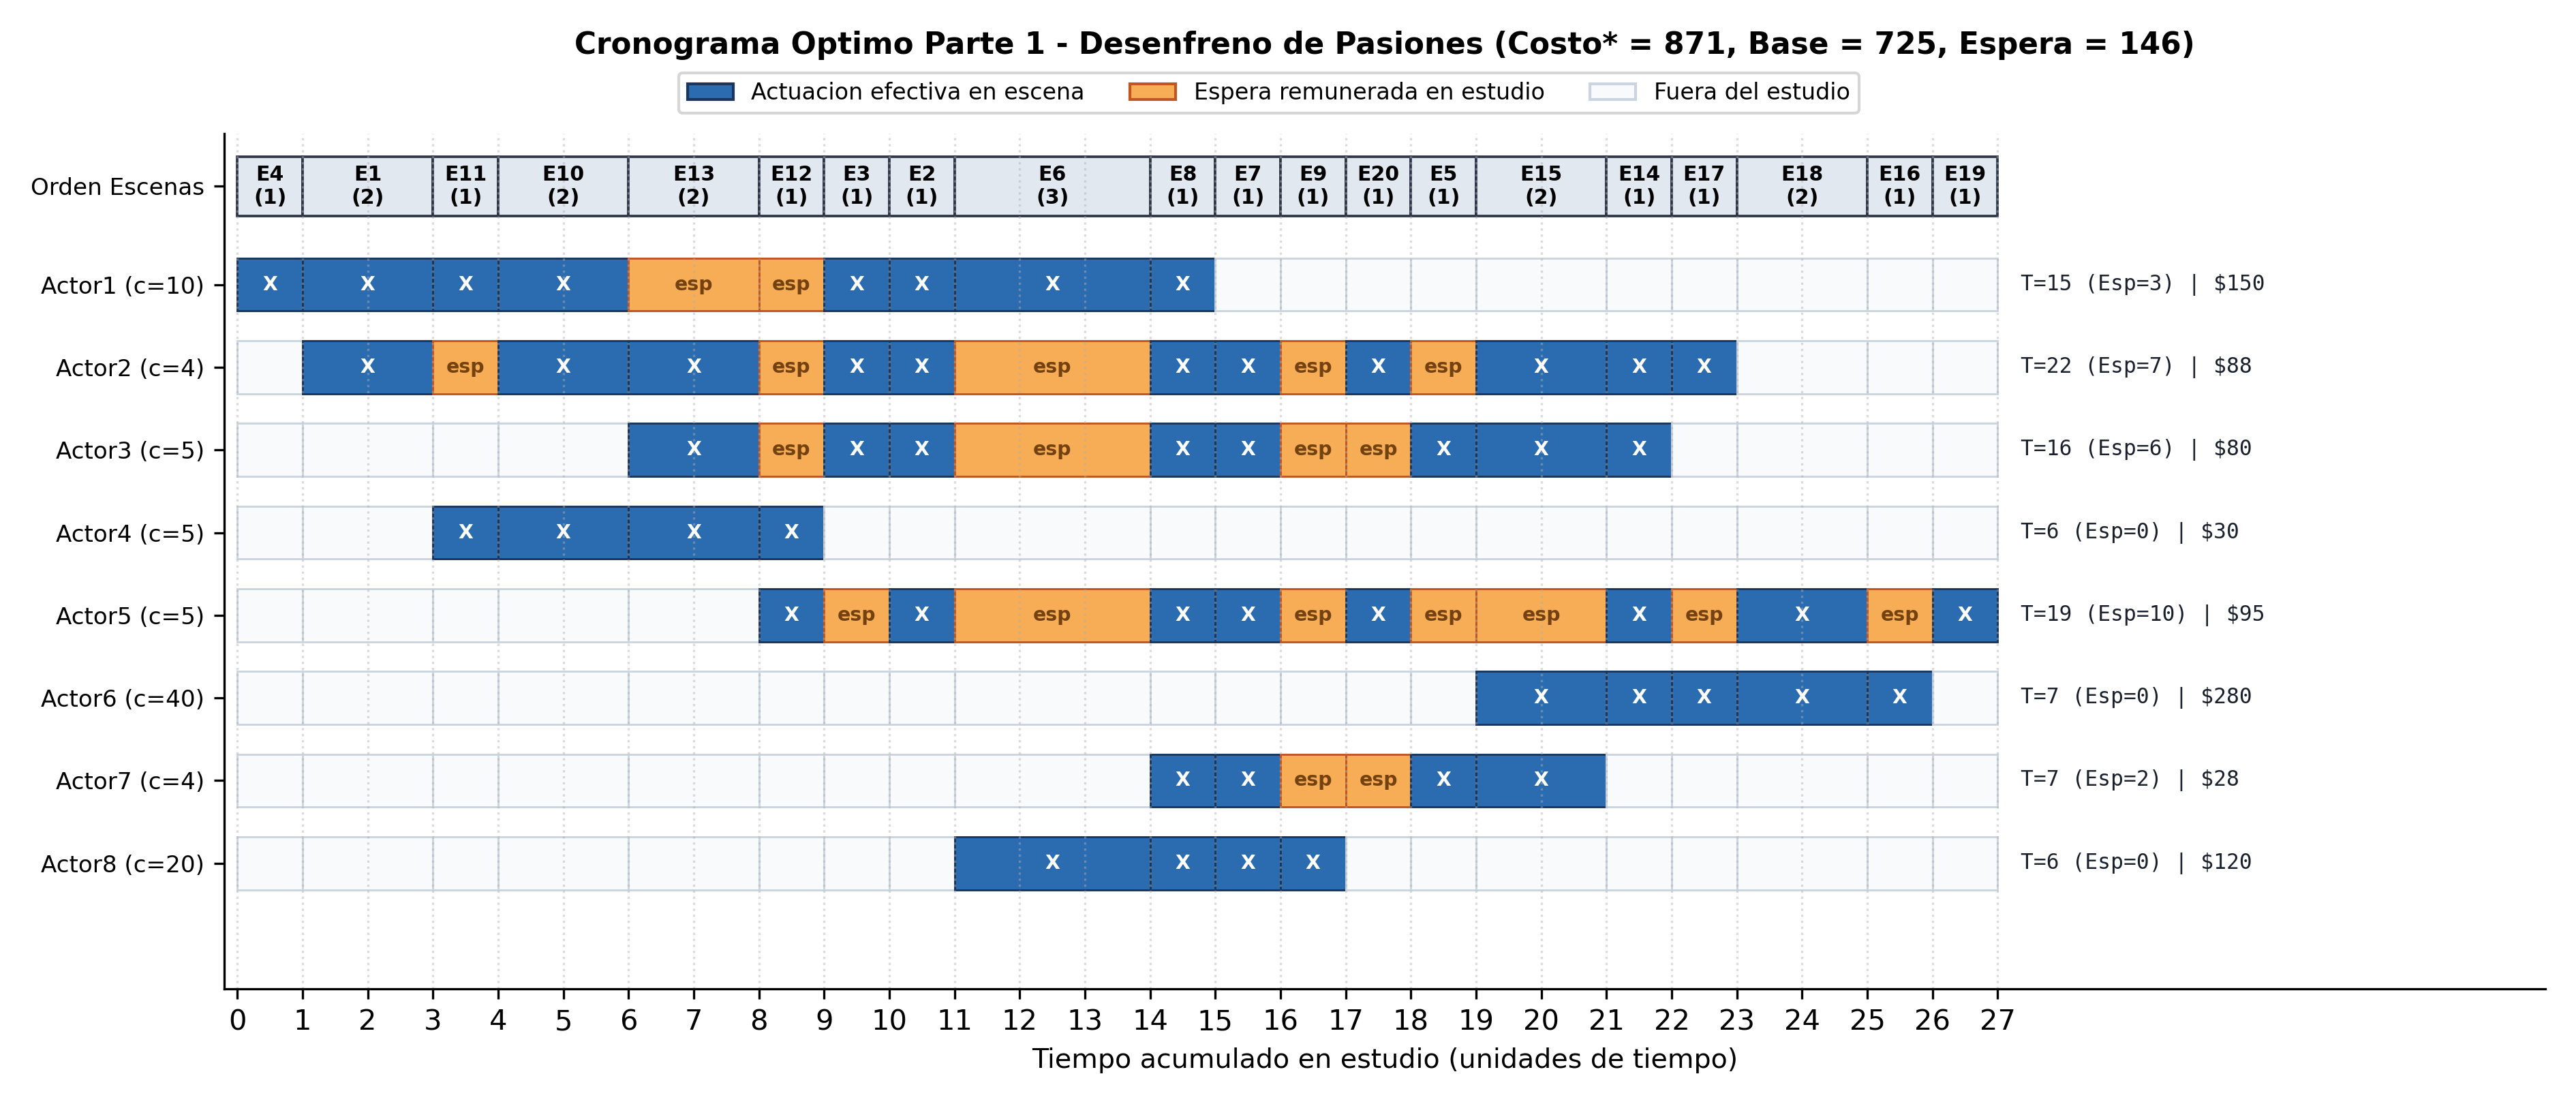
\includegraphics[width=0.90\textwidth]{parte1/gantt_desenfreno_p1.png}
    \caption{Cronograma óptimo de la Parte 1 (\texttt{Desenfreno2.dzn}): $Costo^* = 871$ ($C_{\text{fijo}} = 725$, espera $= 146$) con orden $(4, 1, 11, 10, 13, 12, 3, 2, 6, 8, 7, 9, 20, 5, 15, 14, 17, 18, 16, 19)$.}
    \label{fig:gantt_p1}
\end{figure}

\begin{figure}[!htbp]
    \centering
    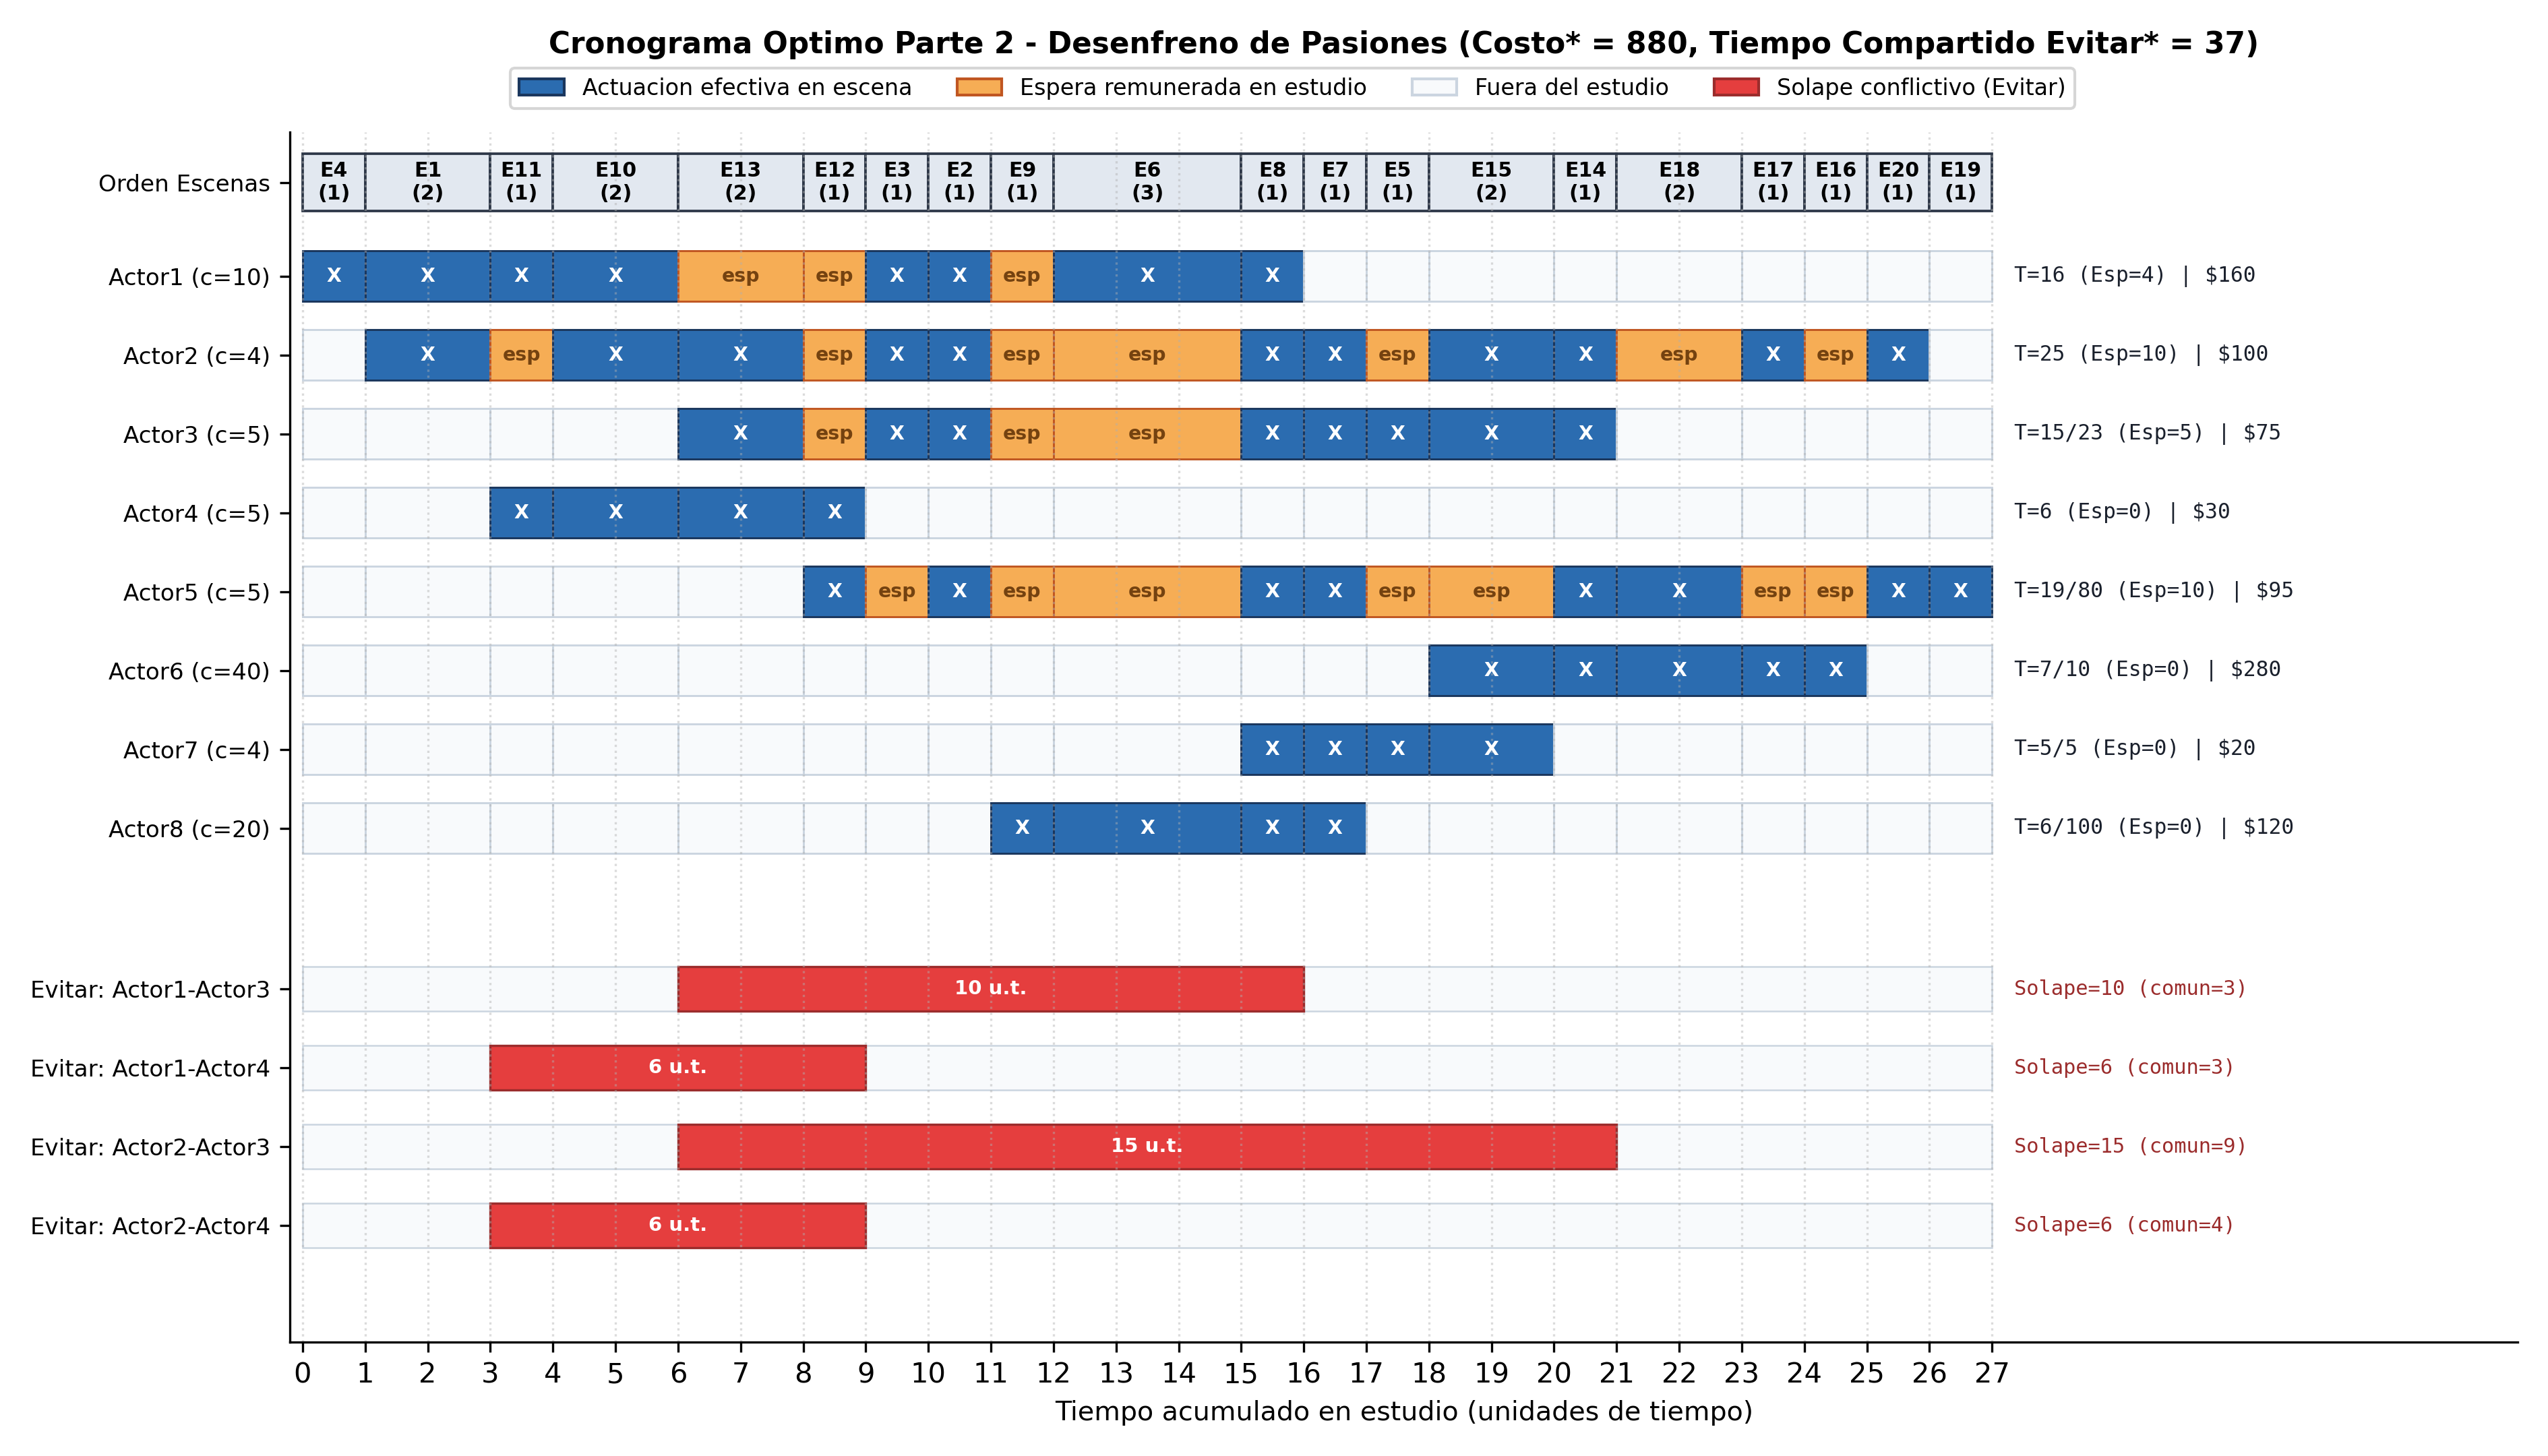
\includegraphics[width=0.90\textwidth]{parte2/gantt_desenfreno_p2_evitar.png}
    \caption{Cronograma óptimo de la Parte 2 (\texttt{Desenfreno4.dzn}): $Costo^* = 880$, $TC^* = 37$ con orden $(4, 1, 11, 10, 13, 12, 3, 2, 9, 6, 8, 7, 5, 15, 14, 18, 17, 16, 20, 19)$.}
    \label{fig:gantt_p2}
\end{figure}

\begin{figure}[!htbp]
    \centering
    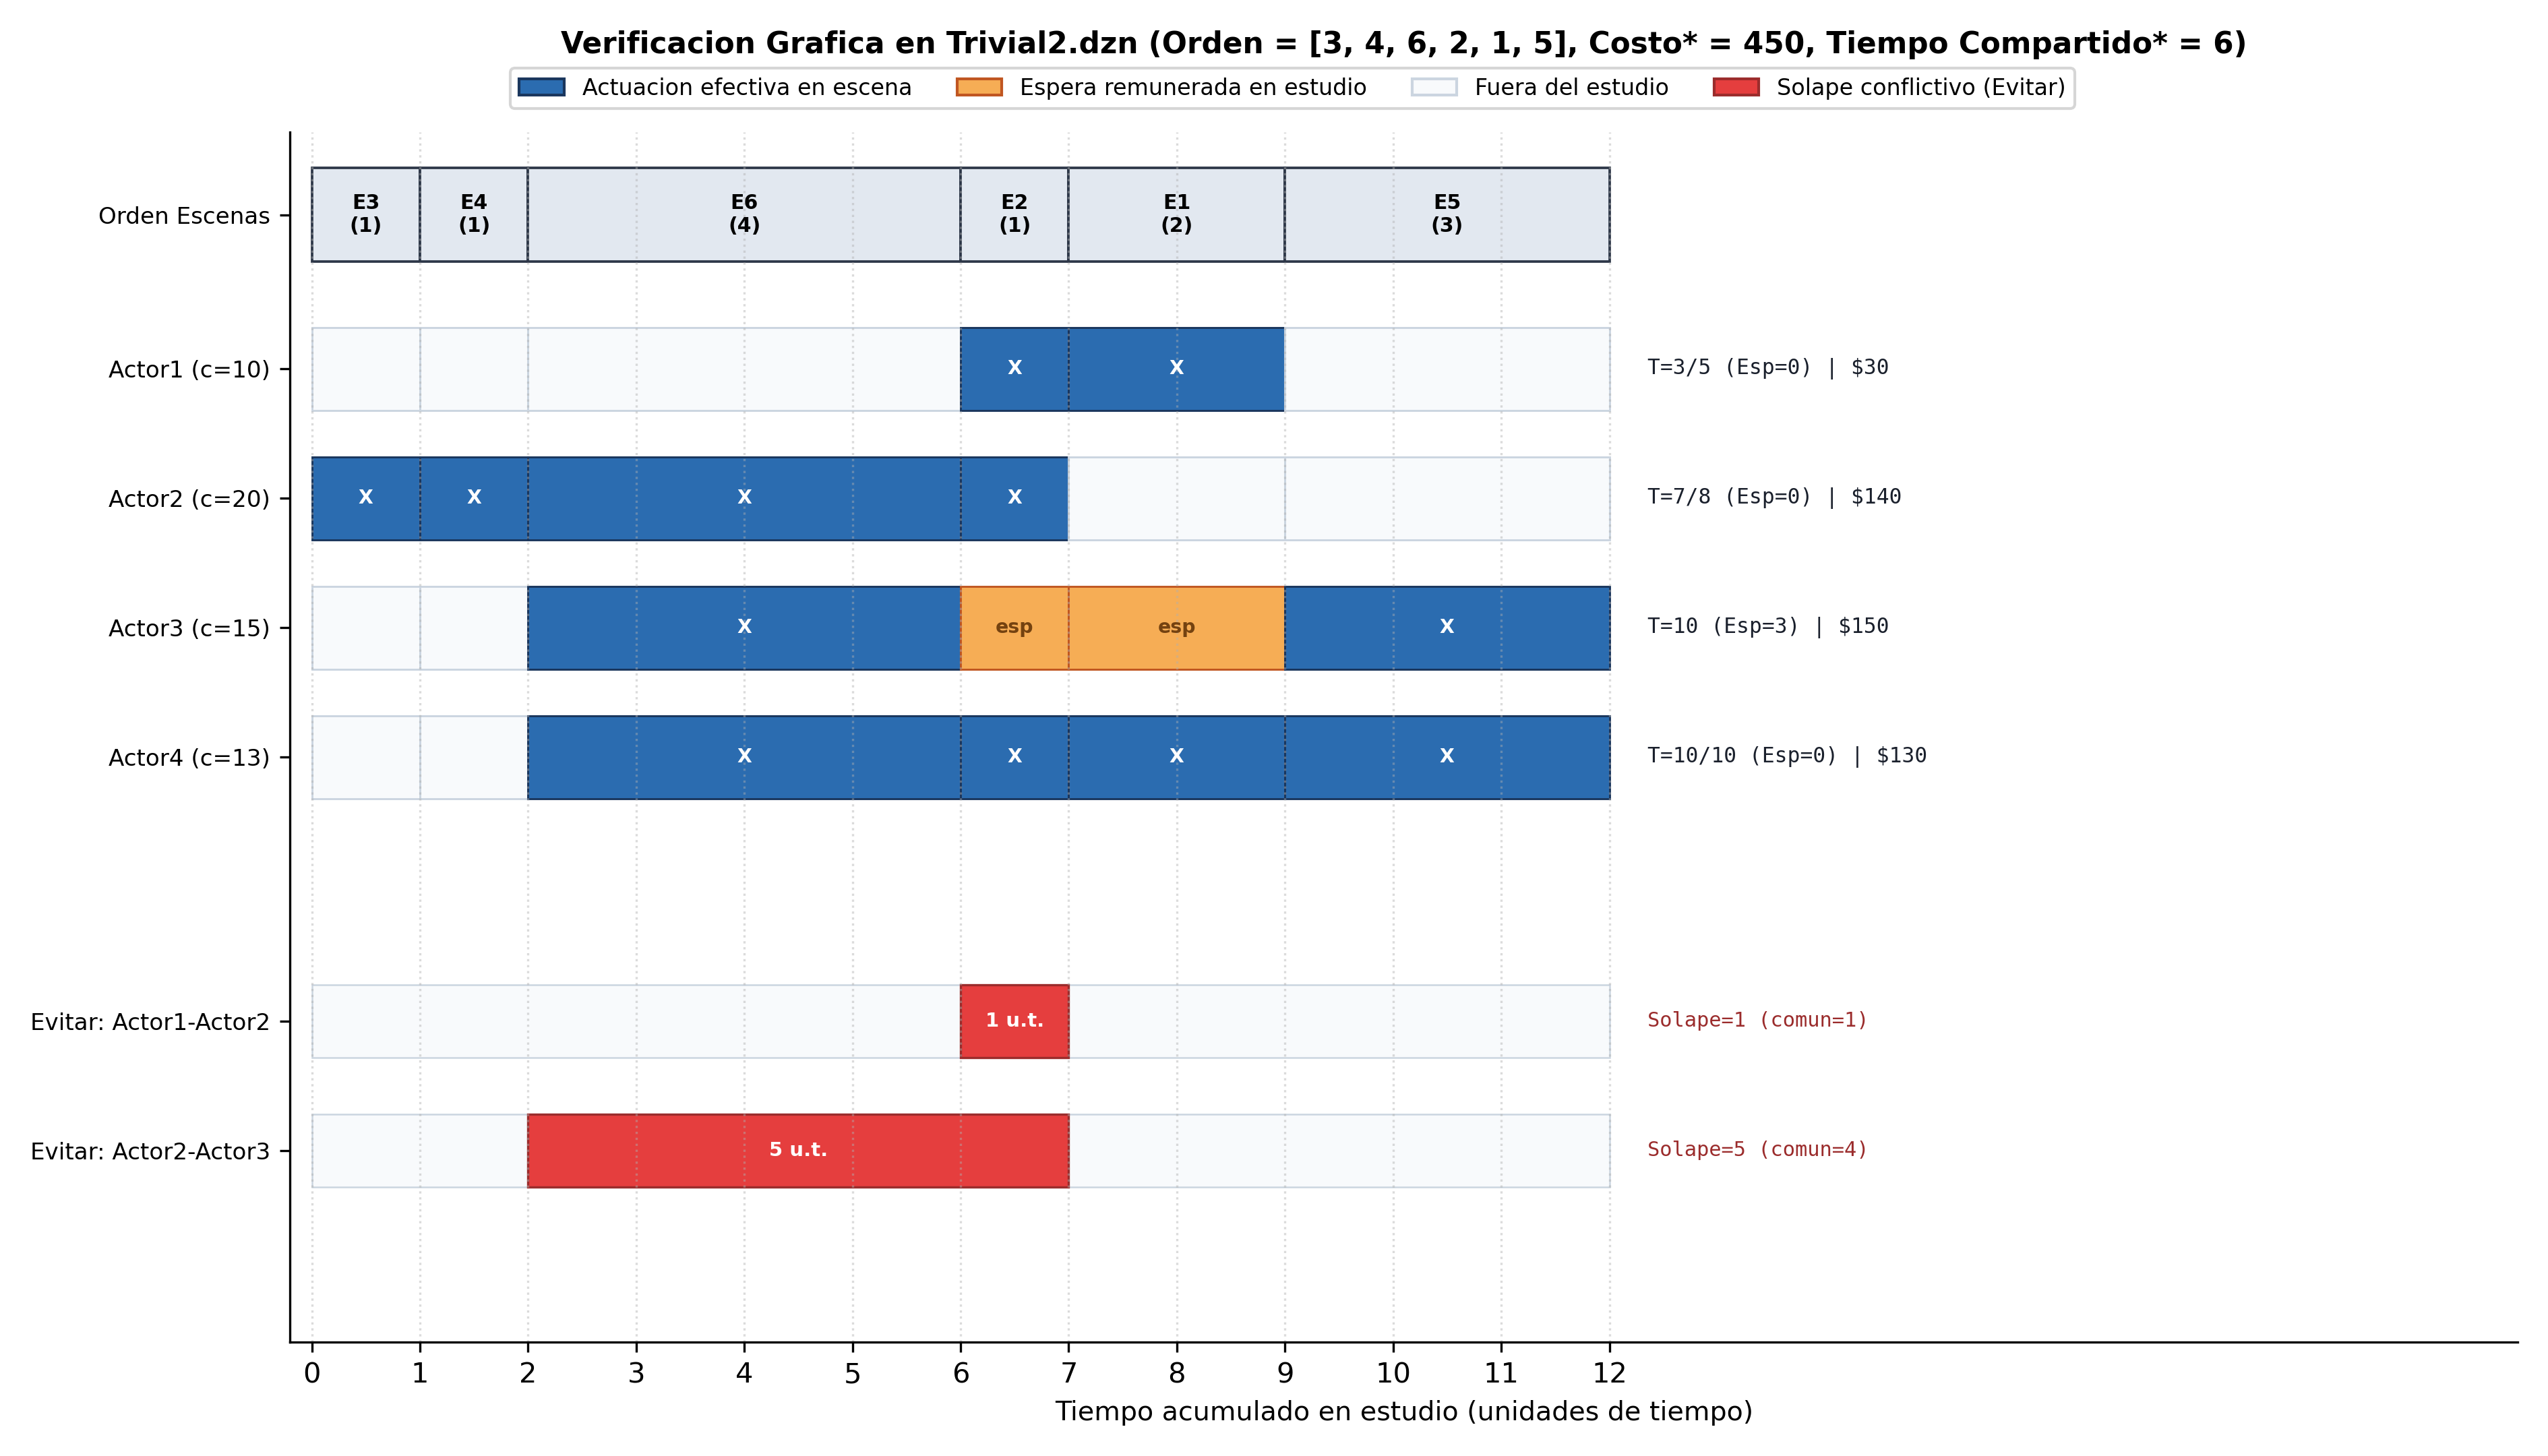
\includegraphics[width=0.86\textwidth]{parte2/verificacion_trivial2_p2.png}
    \caption{Caso base Parte 2 (\texttt{Trivial2.dzn}) con $(Costo^*, TC^*) = (450, 6)$; el orden canónico $(3, 4, 6, 2, 1, 5)$ equivale bajo $S_2$ a $(4, 3, 6, 2, 1, 5)$.}
    \label{fig:gantt_trivial2}
\end{figure}

\begin{itemize}
    \item \textbf{Efecto de \texttt{Disponibilidad}:} En \texttt{Desenfreno2} ($Costo^* = 871$, Figura~\ref{fig:gantt_p1}), los Actores 6 ($c_6 = 40$), 8 ($c_8 = 20$) y 4 ($c_4 = 5$) no tienen esperas, pero el Actor 7 permanece $T_7 = 7$ unidades (espera en $E_9$ y $E_{20}$). En \texttt{Desenfreno4} (Figura~\ref{fig:gantt_p2}), $Disp_7 = 5 = D^{\min}_7$ invalida dicho plan y fuerza a agrupar $[E_8, E_7, E_5, E_{15}]$ en $t \in [15, 20]$, desplazando $E_9$ a $[11, 12]$ y subiendo el óptimo exacto a $Costo^* = 880$ ($+9$ unidades, $\$900\,000$ pesos; análogo a \texttt{Instancia03}: $1531 \to 1544$).
    \item \textbf{Reducción de búsqueda en Parte 2 ($6{,}62\text{ s} \to 1{,}62\text{ s}$):} Pese a sumar variables y criterios, en ``Desenfreno de Pasiones'' los nodos caen $4{,}29\times$ ($71\,753 \to 16\,742$) y los fallos $4{,}45\times$ ($69\,264 \to 15\,582$) porque $R_3$ convierte $Disp_7 = 5$ y $Disp_6 = 10$ en cotas estrechas sobre $ultima_a - primera_a$ desde la raíz.
    \item \textbf{Composición de \texttt{Evitar}:} En \texttt{Desenfreno4}, $\underline{TC} = 3 + 3 + 9 + 4 = 19$ unidades corresponden a escenas compartidas obligatorias; las $18$ restantes hasta $TC^* = 37$ provienen de no separar los bloques de los Actores 1 y 4 respecto a 2 y 3 para no elevar $Costo$ por encima de $880$.
\end{itemize}

\subsection{Ablación: Simetrías vs.\ Modelo Original y Redundantes}

La Tabla~\ref{tab:ablacion} y las Figuras~\ref{fig:ablacion_p1}--\ref{fig:ablacion_p2} comparan el modelo primario original ($M_0$), solo simetrías ($M_1 = M_0 + S_1..S_3$), solo redundantes ($M_2 = M_0 + R_1..R_4$) y el modelo completo ($M_3$).

\begin{table}[!htbp]
\centering
\caption{Ablación ($M_0$ a $M_3$; \texttt{Gecode} para $M \le 12$, \texttt{Chuffed} con límite de $15\text{ s}$ para $M = 20$).}
\label{tab:ablacion}
\resizebox{\textwidth}{!}{%
\setlength{\tabcolsep}{2.8pt}
\begin{tabular}{llrrrrrrrrrrrr}
\toprule
& & \multicolumn{3}{c}{\textbf{$M_0$ (Original)}} & \multicolumn{3}{c}{\textbf{$M_1$ ($+S_1..S_3$)}} & \multicolumn{3}{c}{\textbf{$M_2$ ($+R_1..R_4$)}} & \multicolumn{3}{c}{\textbf{$M_3$ (Completo)}} \\
\cmidrule(lr){3-5} \cmidrule(lr){6-8} \cmidrule(lr){9-11} \cmidrule(lr){12-14}
\textbf{Instancia} & \textbf{Óptimo} & \textbf{Nodos} & \textbf{Fallos} & \textbf{T (s)} & \textbf{Nodos} & \textbf{Fallos} & \textbf{T (s)} & \textbf{Nodos} & \textbf{Fallos} & \textbf{T (s)} & \textbf{Nodos} & \textbf{Fallos} & \textbf{T (s)} \\
\midrule
\texttt{Trivial1}        & $255$       &       11 &       4 & 0,001 &       11 &       4 & 0,001 &        9 &       3 & 0,001 &      9 &      3 & 0,001 \\
\texttt{Instancia01\_P1} & $225$       &      443 &     219 & 0,002 &       26 &      10 & 0,001 &       71 &      32 & 0,001 &     18 &      6 & 0,001 \\
\texttt{Instancia02\_P1} & $871$       &   6\,535 &  3\,250 & 0,028 &   3\,699 &  1\,834 & 0,016 &   1\,136 &     548 & 0,012 &    606 &    286 & 0,007 \\
\texttt{Instancia03\_P1} & $1531$      & 374\,456 & 187\,201 & 1,566 & 181\,709 & 90\,831 & 0,761 &  74\,856 & 37\,400 & 0,667 & 36\,964 & 18\,457 & 0,333 \\
\texttt{Desenfreno2}     & $871$       & 209\,588$^\ddagger$ & 206\,922 & 14,79 & 207\,560$^\ddagger$ & 204\,772 & 14,79 & 121\,572 & 118\,466 & 12,35 & 71\,753 & 69\,264 & 6,596 \\
\midrule
\texttt{Trivial2}        & $(450,6)$   &       55 &      27 & 0,001 &       17 &       8 & 0,001 &       27 &      13 & 0,001 &     11 &      5 & 0,001 \\
\texttt{Instancia01\_P2} & $(225,5)$   &      348 &     165 & 0,002 &      232 &     107 & 0,002 &      220 &     101 & 0,002 &    148 &     65 & 0,002 \\
\texttt{Instancia02\_P2} & $(871,17)$  &   4\,125 &  2\,053 & 0,021 &   2\,637 &  1\,307 & 0,013 &      588 &     284 & 0,006 &    430 &    203 & 0,005 \\
\texttt{Instancia03\_P2} & $(1544,37)$ & 149\,505 & 74\,731 & 0,653 &  71\,767 & 35\,874 & 0,314 &  26\,202 & 13\,079 & 0,239 & 13\,059 &  6\,520 & 0,122 \\
\texttt{Desenfreno4}     & $(880,37)$  & 139\,661$^\ddagger$ & 136\,362 & 14,79 &  92\,992 & 90\,698 & 10,07 &  29\,302 & 27\,743 & 2,727 & 16\,742 & 15\,582 & 1,572 \\
\bottomrule
\multicolumn{14}{l}{\footnotesize $^\ddagger$Halla el valor óptimo pero agota $15\text{ s}$ sin certificar optimalidad.}
\end{tabular}%
}
\end{table}

\begin{figure}[!htbp]
    \centering
    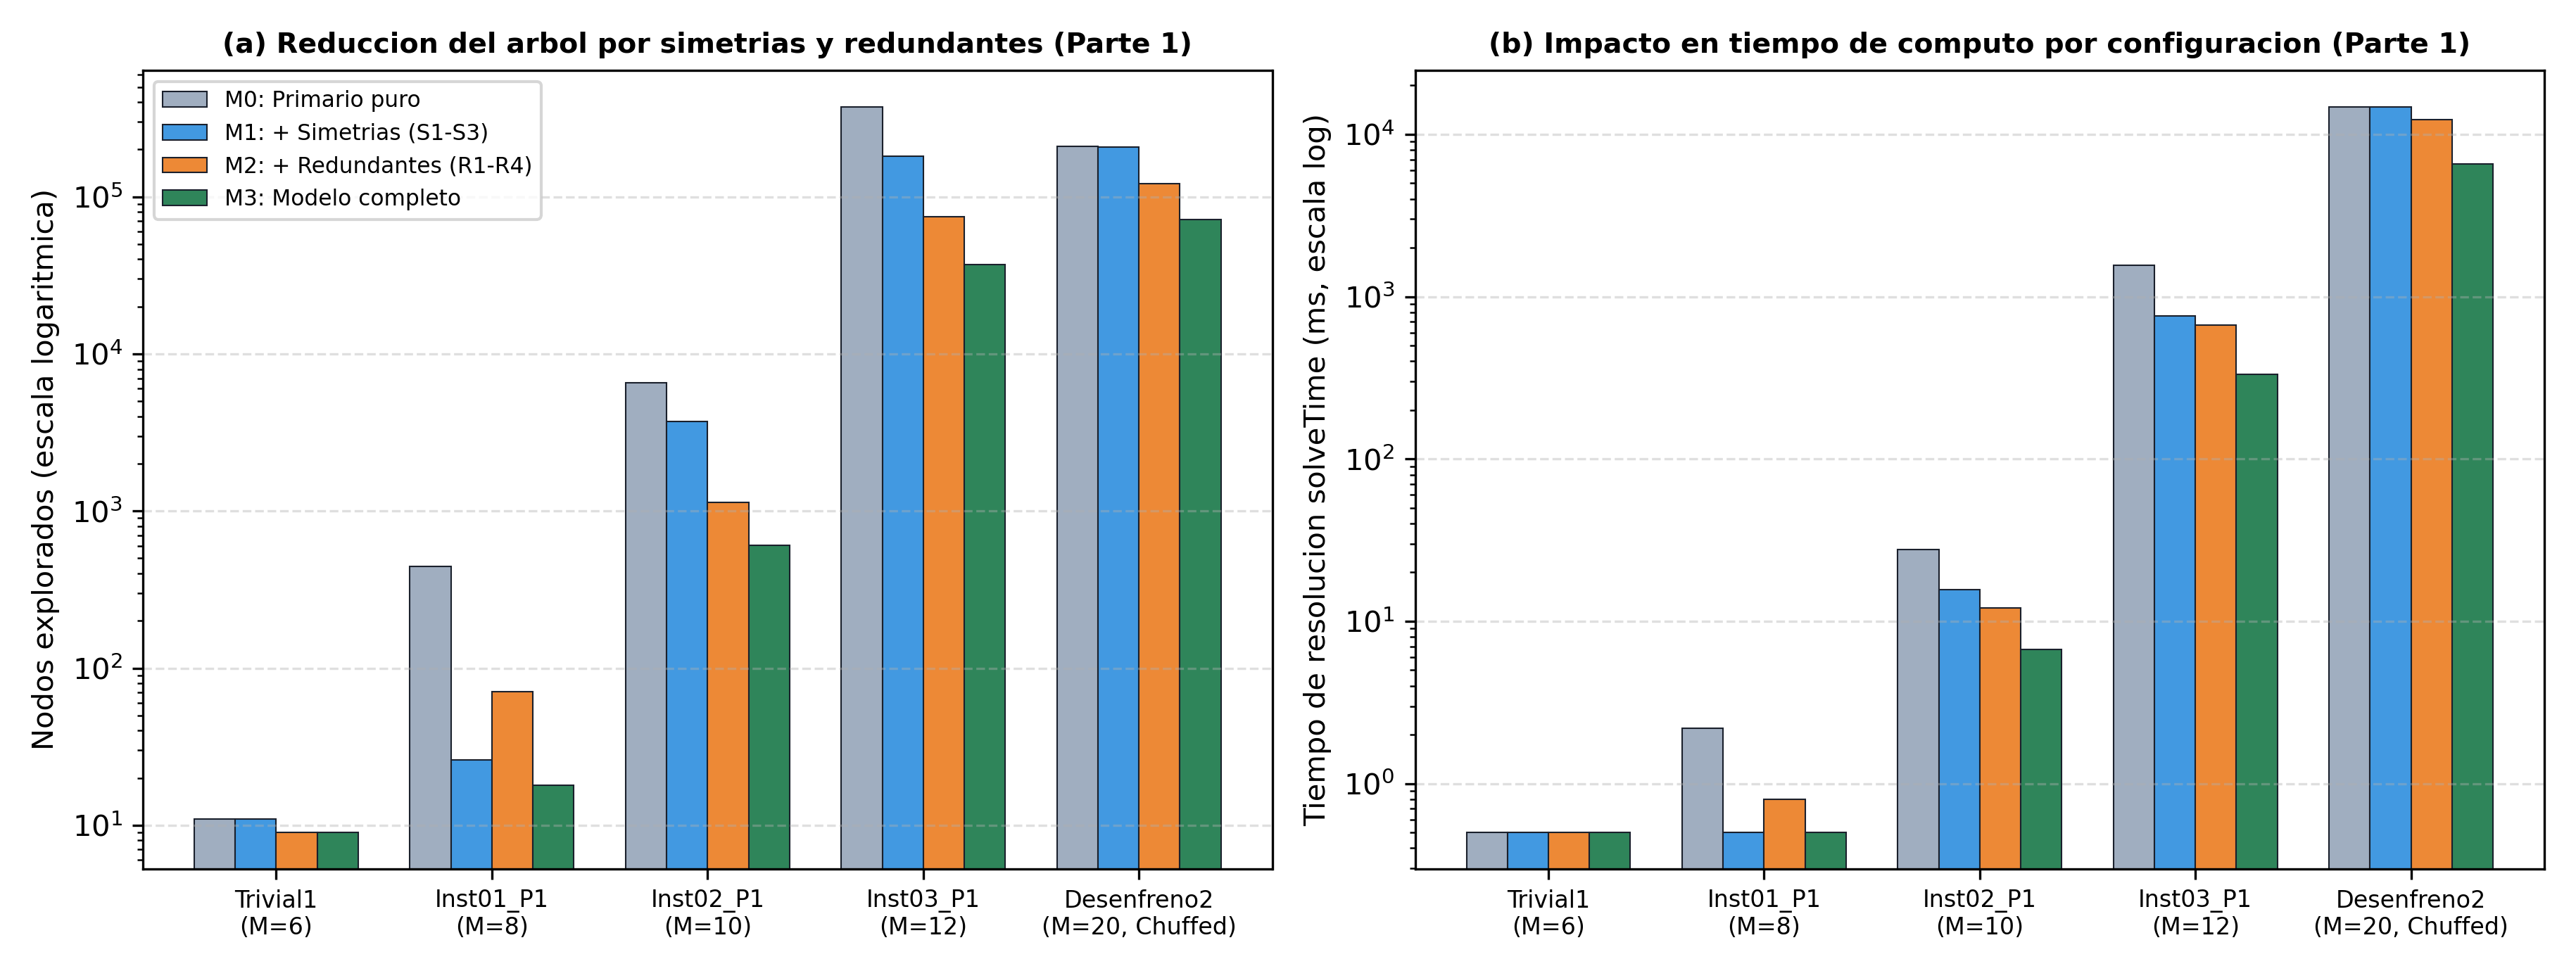
\includegraphics[width=0.83\textwidth]{parte1/ablacion_poda_p1.png}
    \caption{Efecto de las simetrías ($S_1$--$S_3$) y redundantes ($R_1$--$R_4$) sobre nodos y tiempos en la Parte 1.}
    \label{fig:ablacion_p1}
\end{figure}

\begin{figure}[!htbp]
    \centering
    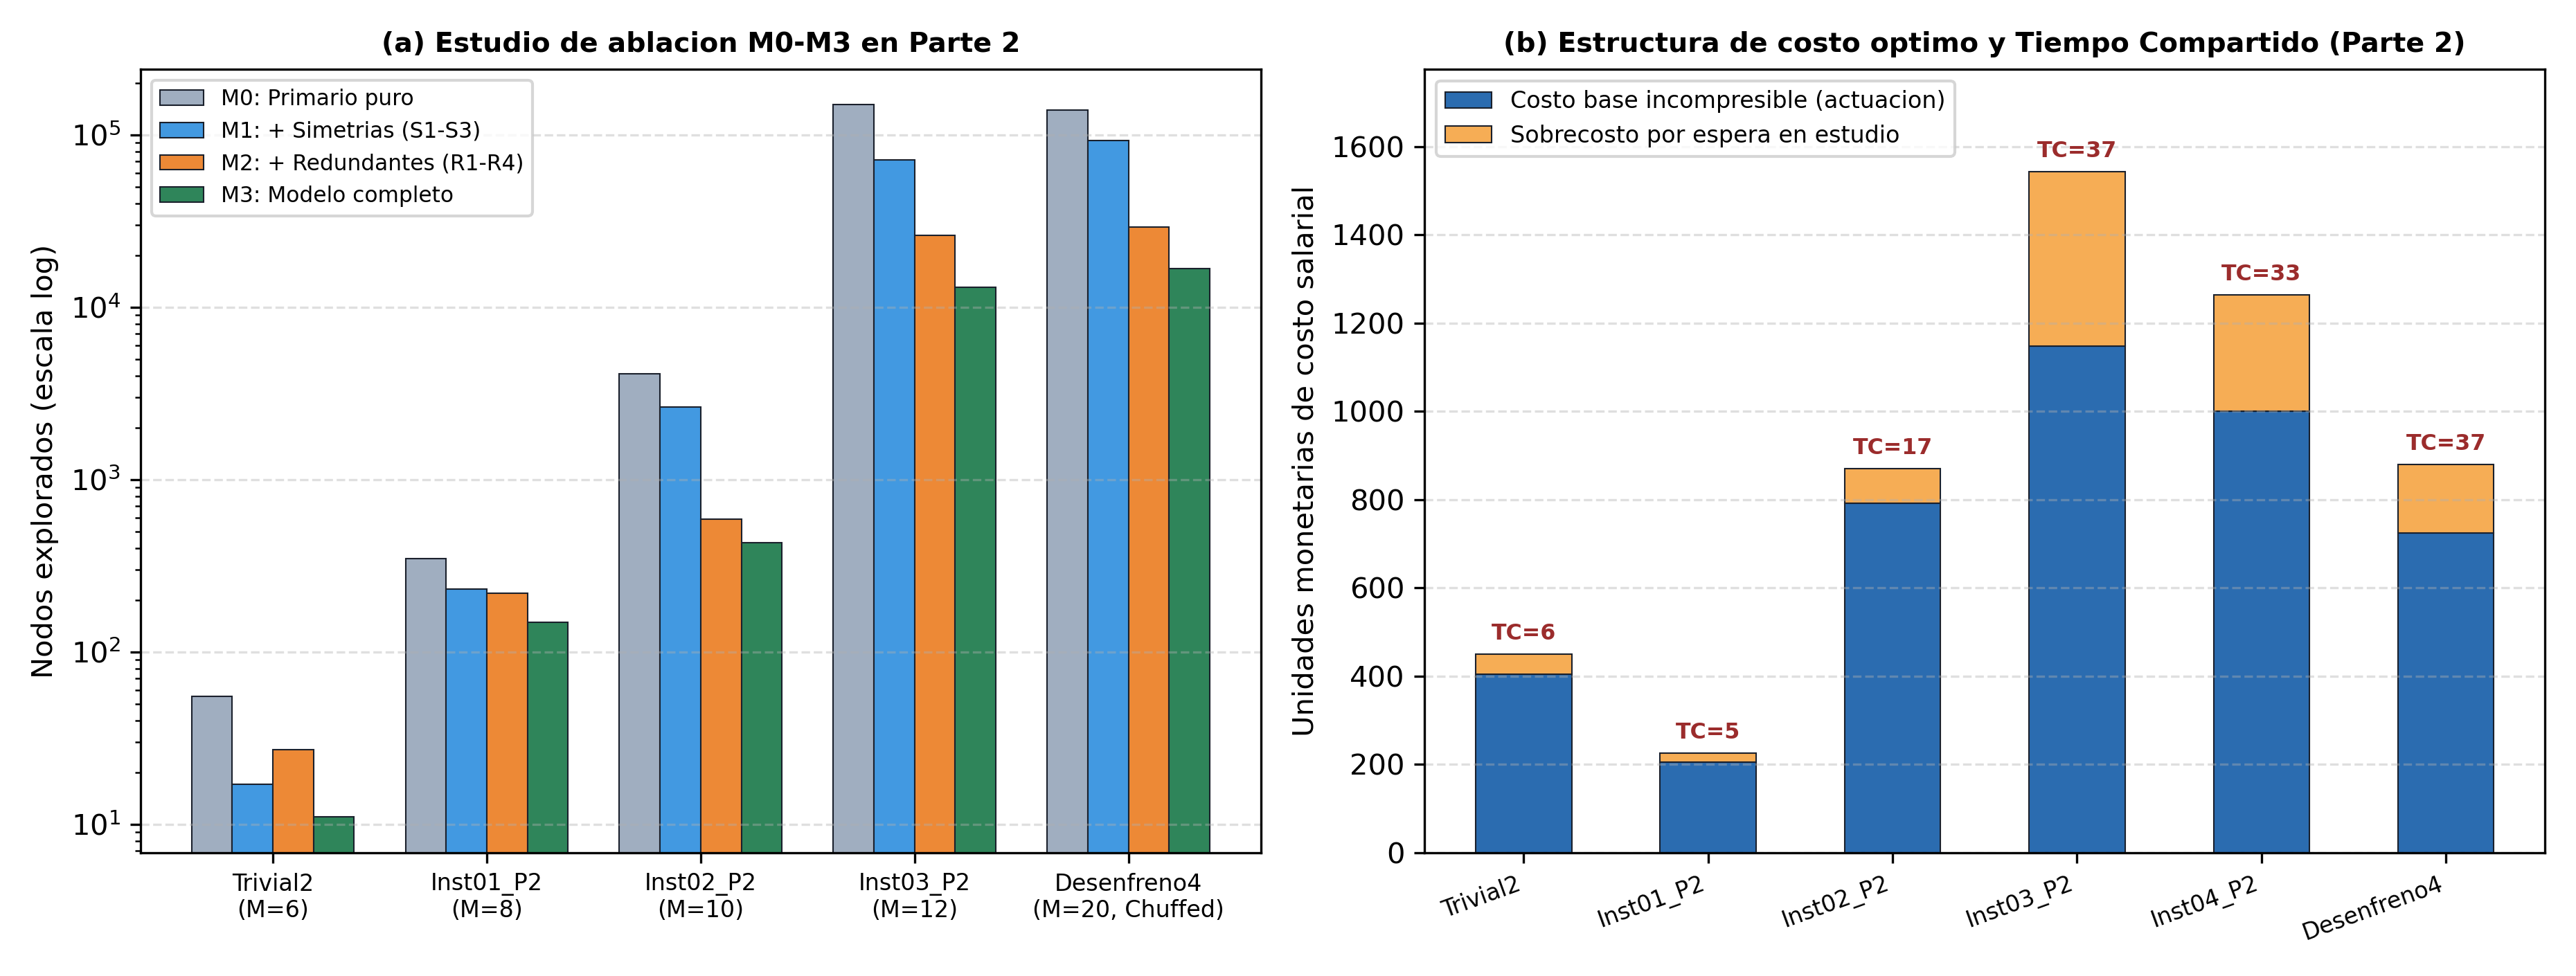
\includegraphics[width=0.83\textwidth]{parte2/ablacion_y_tradeoff_p2.png}
    \caption{Ablación en la Parte 2 y descomposición entre $C_{\text{fijo}}$, espera y tiempo compartido (\texttt{Evitar}).}
    \label{fig:ablacion_p2}
\end{figure}

\begin{itemize}
    \item \textbf{Aporte de simetrías ($M_0 \to M_1$, $M_2 \to M_3$):} Donde solo actúa $S_1$ (\texttt{Instancia03\_P1/P2}), los nodos y fallos se reducen a la mitad ($374\,456 \to 181\,709$, $-51{,}5\%$; $149\,505 \to 71\,767$, $-52{,}0\%$). Con escenas vacías y gemelas, $M_1$ reduce el árbol $17{,}04\times$ en \texttt{Instancia01\_P1} ($443 \to 26$ nodos) y $3{,}24\times$ en \texttt{Trivial2} ($55 \to 17$), y en \texttt{Desenfreno4} logra certificar optimalidad en $10{,}07\text{ s}$ frente al corte por tiempo de $M_0$.
    \item \textbf{Combinación con redundantes ($M_3$):} En \texttt{Desenfreno2}, $M_0$ y $M_1$ agotan $15\text{ s}$ sin prueba de optimalidad; $R_1$--$R_4$ ($M_2$) cierran la prueba en $12{,}35\text{ s}$ y $M_3$ la baja a $6{,}60\text{ s}$, con reducciones totales de $24{,}61\times$ (\texttt{Instancia01\_P1}), $10{,}13\times$ (\texttt{Instancia03\_P1}), $11{,}45\times$ (\texttt{Instancia03\_P2}) y $8{,}34\times$ en nodos ($9{,}41\times$ en tiempo) sobre \texttt{Desenfreno4}.
\end{itemize}

\subsection{Comparación de Estrategias de Búsqueda (\texorpdfstring{$E_1$--$E_8$}{E1-E8})}

La Tabla~\ref{tab:estrategias} y la Figura~\ref{fig:estrategias} contrastan $E_1$--$E_8$ con límite de $8{,}5\text{ s}$ por corrida.

\begin{table}[!htbp]
\centering
\caption{Comparación de las estrategias $E_1$--$E_8$ en $M=12$ (\texttt{Gecode} y \texttt{Chuffed}) y $M=20$ (\texttt{Chuffed}, límite $8{,}5\text{ s}$).}
\label{tab:estrategias}
\resizebox{\textwidth}{!}{%
\setlength{\tabcolsep}{2.4pt}
\begin{tabular}{llrrrrrrrrrrrrrr}
\toprule
& & \multicolumn{3}{c}{\textbf{Inst03\_P1 (Gecode)}} & \multicolumn{3}{c}{\textbf{Inst03\_P1 (Chuffed)}} & \multicolumn{4}{c}{\textbf{Desenfreno2 (Chuffed)}} & \multicolumn{4}{c}{\textbf{Desenfreno4 (Chuffed)}} \\
\cmidrule(lr){3-5} \cmidrule(lr){6-8} \cmidrule(lr){9-12} \cmidrule(lr){13-16}
\textbf{ID} & \textbf{Estrategia} & \textbf{Nodos} & \textbf{Fallos} & \textbf{T (s)} & \textbf{Nodos} & \textbf{Fallos} & \textbf{T (s)} & \textbf{Costo} & \textbf{Nodos} & \textbf{Fallos} & \textbf{T (s)} & \textbf{Par} & \textbf{Nodos} & \textbf{Fallos} & \textbf{T (s)} \\
\midrule
$E_1$ & Out-In Peso Asc    &  36\,964 &  18\,457 & 0,335 &  4\,049 &  3\,786 & 0,147 & \textbf{871}$\checkmark$ &  71\,753 & 69\,264 & \textbf{6,676} & \textbf{(880,37)}$\checkmark$ &  16\,742 & 15\,582 & \textbf{1,592} \\
$E_2$ & Out-In ID Nominal  &  47\,716 &  23\,809 & 0,375 &  5\,650 &  5\,166 & 0,195 & 871$^*$                  &  98\,608 & 94\,538 & 8,262          & (880,37)$\checkmark$          &  40\,289 & 38\,085 & 3,916 \\
$E_3$ & Izquierda-Derecha  & 785\,034$^*$ & 392\,451 & 8,290 & 66\,907 & 66\,234 & 4,282 & 925$^*$              &  71\,174 & 70\,841 & 8,275          & (899,45)$^*$                  &  63\,829 & 62\,550 & 8,278 \\
$E_4$ & First-Fail + Min   & 440\,476 & 220\,173 & 4,230 & 22\,645 & 21\,971 & 1,126 & 925$^*$                  &  72\,526 & 71\,788 & 8,281          & (880,37)$\checkmark$          &  75\,862 & 73\,078 & 8,023 \\
$E_5$ & First-Fail + Split & 438\,673 & 219\,270 & 3,829 & 26\,767 & 23\,648 & 1,249 & 925$^*$                  &  78\,591 & 65\,207 & 8,276          & (880,37)$\checkmark$          &  85\,669 & 72\,754 & 7,834 \\
$E_6$ & Pos Costo + Med    & 582\,417$^*$ & 291\,174 & 8,292 & 94\,318$^*$ & 93\,915 & 8,277 & 1049$^*$          &  77\,915 & 76\,985 & 8,280          & (970,41)$^*$                  &  70\,750 & 69\,748 & 8,272 \\
$E_7$ & Dom/WDeg Out-In    &  36\,956 &  18\,453 & 0,337 &  4\,049 &  3\,786 & 0,147 & \textbf{871}$\checkmark$ &  71\,753 & 69\,264 & 6,714          & \textbf{(880,37)}$\checkmark$ &  16\,742 & 15\,582 & 1,538 \\
$E_8$ & Default Solver     & 146\,445 &  73\,167 & 1,168 & 161\,833$^*$ & 116\,481 & 8,295 & 1046$^*$           & 143\,053 & 87\,742 & 8,281          & (1094,48)$^*$                 & 132\,022 & 76\,344 & 8,279 \\
\bottomrule
\multicolumn{16}{l}{\footnotesize $\checkmark$ Optimalidad certificada (\texttt{==========}). \quad $^*$Agota $8{,}5\text{ s}$ sin certificar optimalidad.}
\end{tabular}%
}
\end{table}

\begin{figure}[!htbp]
    \centering
    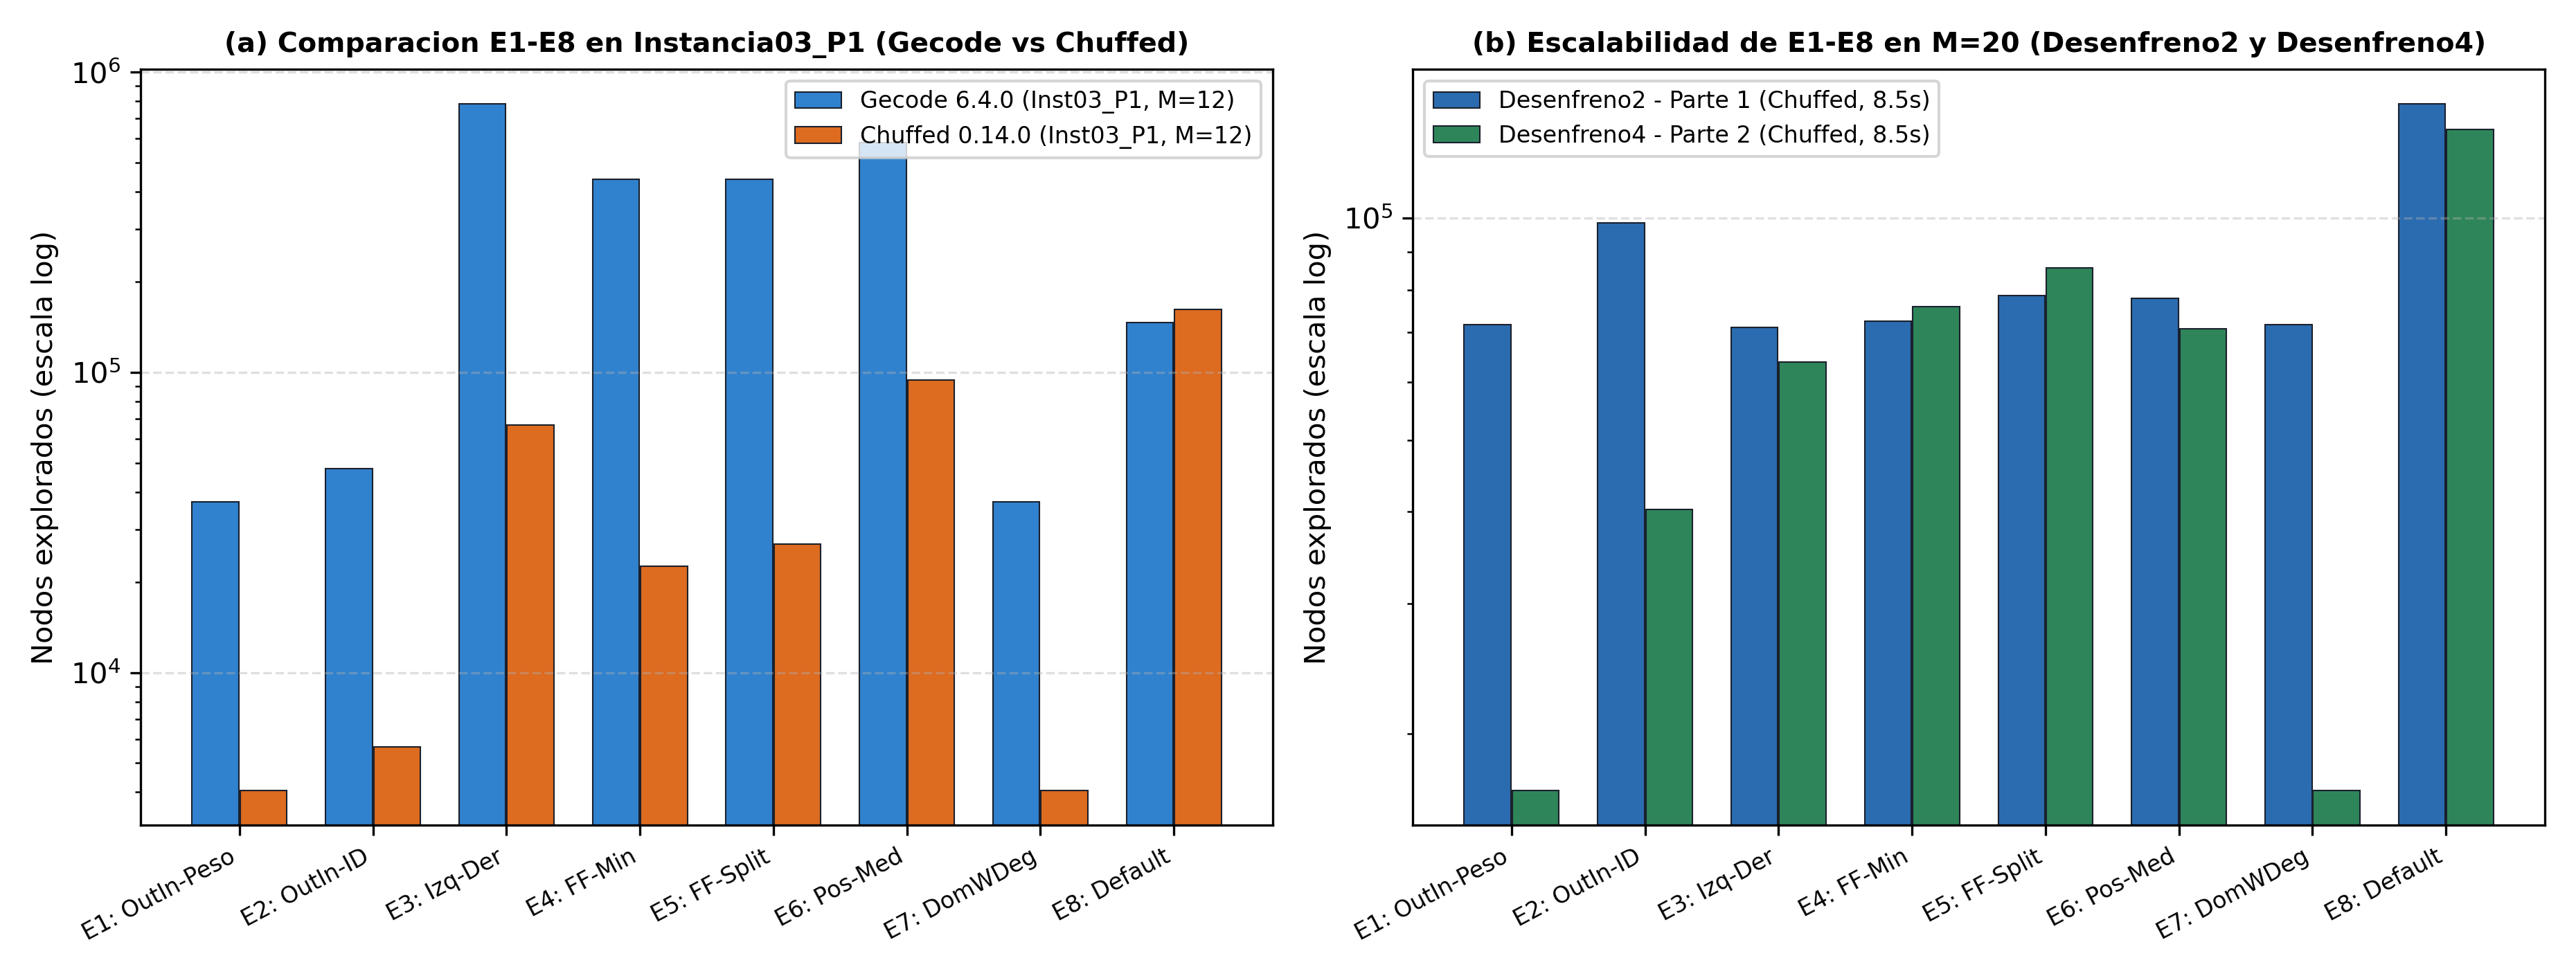
\includegraphics[width=0.82\textwidth]{parte1/estrategias_busqueda_p1.png}
    \caption{Nodos explorados por las estrategias $E_1$--$E_8$ en $M=12$ (\texttt{Gecode} y \texttt{Chuffed}) y $M=20$ (\texttt{Chuffed}).}
    \label{fig:estrategias}
\end{figure}

\begin{itemize}
    \item \textbf{Limitación de la búsqueda por defecto ($E_8$):} En \texttt{Gecode} explora $3{,}96\times$ más nodos y fallos que $E_1$; en \texttt{Chuffed} agota el tiempo incluso en $M=12$, y en $M=20$ se estanca en $Costo = 1046$ (\texttt{Desenfreno2}) y $(1094, 48)$ (\texttt{Desenfreno4}), lejos de $871$ y $(880, 37)$.
    \item \textbf{Efecto del orden \emph{Outside-In} ($E_3 \to E_2$) y del peso salarial ($E_2 \to E_1$):} Pasar de izquierda-a-derecha ($E_3$) a extremos intercalados ($E_2$) en \texttt{Instancia03\_P1} reduce $11{,}84\times$ los nodos y $21{,}96\times$ el tiempo en \texttt{Chuffed}. Ordenar además los valores por $W_e$ ascendente ($E_1$, igualada por $E_7$) recorta $2{,}41\times$ los nodos en \texttt{Desenfreno4} ($40\,289 \to 16\,742$) y permite certificar \texttt{Desenfreno2} en $6{,}68\text{ s}$.
    \item \textbf{\texttt{Chuffed} vs.\ \texttt{Gecode}:} Distintos prefijos y sufijos generan el mismo conjunto de actores abiertos en el bloque central; mientras \texttt{Gecode} re-explora subárboles equivalentes por DFS (razón nodos/fallos $\approx 2{:}1$), \texttt{Chuffed} aprende cláusulas \emph{nogood} sobre literales de orden e intermediación, reduciendo entre $9\times$ y $46\times$ los nodos para $M \ge 12$.
\end{itemize}
